\documentclass[twoside]{book}

% Packages required by doxygen
\usepackage{fixltx2e}
\usepackage{calc}
\usepackage{doxygen}
\usepackage[export]{adjustbox} % also loads graphicx
\usepackage{graphicx}
\usepackage[utf8]{inputenc}
\usepackage{makeidx}
\usepackage{multicol}
\usepackage{multirow}
\PassOptionsToPackage{warn}{textcomp}
\usepackage{textcomp}
\usepackage[nointegrals]{wasysym}
\usepackage[table]{xcolor}

% Font selection
\usepackage[T1]{fontenc}
\usepackage[scaled=.90]{helvet}
\usepackage{courier}
\usepackage{amssymb}
\usepackage{sectsty}
\renewcommand{\familydefault}{\sfdefault}
\allsectionsfont{%
  \fontseries{bc}\selectfont%
  \color{darkgray}%
}
\renewcommand{\DoxyLabelFont}{%
  \fontseries{bc}\selectfont%
  \color{darkgray}%
}
\newcommand{\+}{\discretionary{\mbox{\scriptsize$\hookleftarrow$}}{}{}}

% Page & text layout
\usepackage{geometry}
\geometry{%
  a4paper,%
  top=2.5cm,%
  bottom=2.5cm,%
  left=2.5cm,%
  right=2.5cm%
}
\tolerance=750
\hfuzz=15pt
\hbadness=750
\setlength{\emergencystretch}{15pt}
\setlength{\parindent}{0cm}
\setlength{\parskip}{3ex plus 2ex minus 2ex}
\makeatletter
\renewcommand{\paragraph}{%
  \@startsection{paragraph}{4}{0ex}{-1.0ex}{1.0ex}{%
    \normalfont\normalsize\bfseries\SS@parafont%
  }%
}
\renewcommand{\subparagraph}{%
  \@startsection{subparagraph}{5}{0ex}{-1.0ex}{1.0ex}{%
    \normalfont\normalsize\bfseries\SS@subparafont%
  }%
}
\makeatother

% Headers & footers
\usepackage{fancyhdr}
\pagestyle{fancyplain}
\fancyhead[LE]{\fancyplain{}{\bfseries\thepage}}
\fancyhead[CE]{\fancyplain{}{}}
\fancyhead[RE]{\fancyplain{}{\bfseries\leftmark}}
\fancyhead[LO]{\fancyplain{}{\bfseries\rightmark}}
\fancyhead[CO]{\fancyplain{}{}}
\fancyhead[RO]{\fancyplain{}{\bfseries\thepage}}
\fancyfoot[LE]{\fancyplain{}{}}
\fancyfoot[CE]{\fancyplain{}{}}
\fancyfoot[RE]{\fancyplain{}{\bfseries\scriptsize Generated by Doxygen }}
\fancyfoot[LO]{\fancyplain{}{\bfseries\scriptsize Generated by Doxygen }}
\fancyfoot[CO]{\fancyplain{}{}}
\fancyfoot[RO]{\fancyplain{}{}}
\renewcommand{\footrulewidth}{0.4pt}
\renewcommand{\chaptermark}[1]{%
  \markboth{#1}{}%
}
\renewcommand{\sectionmark}[1]{%
  \markright{\thesection\ #1}%
}

% Indices & bibliography
\usepackage{natbib}
\usepackage[titles]{tocloft}
\setcounter{tocdepth}{3}
\setcounter{secnumdepth}{5}
\makeindex

% Hyperlinks (required, but should be loaded last)
\usepackage{ifpdf}
\ifpdf
  \usepackage[pdftex,pagebackref=true]{hyperref}
\else
  \usepackage[ps2pdf,pagebackref=true]{hyperref}
\fi
\hypersetup{%
  colorlinks=true,%
  linkcolor=blue,%
  citecolor=blue,%
  unicode%
}

% Custom commands
\newcommand{\clearemptydoublepage}{%
  \newpage{\pagestyle{empty}\cleardoublepage}%
}

\usepackage{caption}
\captionsetup{labelsep=space,justification=centering,font={bf},singlelinecheck=off,skip=4pt,position=top}

%===== C O N T E N T S =====

\begin{document}

% Titlepage & ToC
\hypersetup{pageanchor=false,
             bookmarksnumbered=true,
             pdfencoding=unicode
            }
\pagenumbering{roman}
\begin{titlepage}
\vspace*{7cm}
\begin{center}%
{\Large My Project }\\
\vspace*{1cm}
{\large Generated by Doxygen 1.8.11}\\
\end{center}
\end{titlepage}
\clearemptydoublepage
\tableofcontents
\clearemptydoublepage
\pagenumbering{arabic}
\hypersetup{pageanchor=true}

%--- Begin generated contents ---
\chapter{File Index}
\section{File List}
Here is a list of all files with brief descriptions\+:\begin{DoxyCompactList}
\item\contentsline{section}{\hyperlink{Lab1_8c}{Lab1.\+c} }{\pageref{Lab1_8c}}{}
\end{DoxyCompactList}

\chapter{File Documentation}
\hypertarget{Selection_8c}{}\section{Selection.\+c File Reference}
\label{Selection_8c}\index{Selection.\+c@{Selection.\+c}}
{\ttfamily \#include $<$stdio.\+h$>$}\\*
Include dependency graph for Selection.\+c\+:
\nopagebreak
\begin{figure}[H]
\begin{center}
\leavevmode
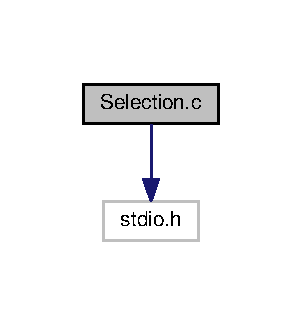
\includegraphics[width=145pt]{Selection_8c__incl}
\end{center}
\end{figure}
\subsection*{Macros}
\begin{DoxyCompactItemize}
\item 
\#define \hyperlink{Selection_8c_a5de5d183f9a6a8d53316f743e1ca6dc2}{N\+M\+AX}~10
\end{DoxyCompactItemize}
\subsection*{Functions}
\begin{DoxyCompactItemize}
\item 
int \hyperlink{Selection_8c_a536581ae21f83a263a18561a10c9ce3d}{get\+Int\+Array} (int nmax, int a\mbox{[}nmax\mbox{]}, int sentinel)
\item 
void \hyperlink{Selection_8c_a8f37fcbee658573c44964f9271a48d5d}{print\+Int\+Array} (int n, int a\mbox{[}$\,$\mbox{]})
\item 
void \hyperlink{Selection_8c_acc86466d0607ef8c19c7d748904206e7}{selection\+Sort} (int n, int a\mbox{[}$\,$\mbox{]})
\item 
int \hyperlink{Selection_8c_a840291bc02cba5474a4cb46a9b9566fe}{main} (void)
\item 
void \hyperlink{Selection_8c_a5ea4efa90d2fa03117a98b554d75be66}{print\+Int\+Array} (int n, int a\mbox{[}n\mbox{]})
\end{DoxyCompactItemize}


\subsection{Macro Definition Documentation}
\index{Selection.\+c@{Selection.\+c}!N\+M\+AX@{N\+M\+AX}}
\index{N\+M\+AX@{N\+M\+AX}!Selection.\+c@{Selection.\+c}}
\subsubsection[{\texorpdfstring{N\+M\+AX}{NMAX}}]{\setlength{\rightskip}{0pt plus 5cm}\#define N\+M\+AX~10}\hypertarget{Selection_8c_a5de5d183f9a6a8d53316f743e1ca6dc2}{}\label{Selection_8c_a5de5d183f9a6a8d53316f743e1ca6dc2}


\subsection{Function Documentation}
\index{Selection.\+c@{Selection.\+c}!get\+Int\+Array@{get\+Int\+Array}}
\index{get\+Int\+Array@{get\+Int\+Array}!Selection.\+c@{Selection.\+c}}
\subsubsection[{\texorpdfstring{get\+Int\+Array(int nmax, int a[nmax], int sentinel)}{getIntArray(int nmax, int a[nmax], int sentinel)}}]{\setlength{\rightskip}{0pt plus 5cm}int get\+Int\+Array (
\begin{DoxyParamCaption}
\item[{int}]{nmax, }
\item[{int}]{a\mbox{[}nmax\mbox{]}, }
\item[{int}]{sentinel}
\end{DoxyParamCaption}
)}\hypertarget{Selection_8c_a536581ae21f83a263a18561a10c9ce3d}{}\label{Selection_8c_a536581ae21f83a263a18561a10c9ce3d}

\begin{DoxyCode}
56 \{
57   \textcolor{keywordtype}{int} n = 0;
58   \textcolor{keywordtype}{int} temp;
59 
60   \textcolor{keywordflow}{do} \{
61     printf(\textcolor{stringliteral}{"Enter integer [%d to terminate] : "}, sentinel);
62     scanf(\textcolor{stringliteral}{"%d"}, &temp);
63     \textcolor{keywordflow}{if} (temp==sentinel) \textcolor{keywordflow}{break};
64     \textcolor{keywordflow}{if} (n==nmax)
65       printf(\textcolor{stringliteral}{"array is full\(\backslash\)n"});
66     \textcolor{keywordflow}{else} 
67       a[n++] = temp;
68   \}\textcolor{keywordflow}{while} (1);
69   \textcolor{keywordflow}{return} n;
70 \}
\end{DoxyCode}
\index{Selection.\+c@{Selection.\+c}!main@{main}}
\index{main@{main}!Selection.\+c@{Selection.\+c}}
\subsubsection[{\texorpdfstring{main(void)}{main(void)}}]{\setlength{\rightskip}{0pt plus 5cm}int main (
\begin{DoxyParamCaption}
\item[{void}]{}
\end{DoxyParamCaption}
)}\hypertarget{Selection_8c_a840291bc02cba5474a4cb46a9b9566fe}{}\label{Selection_8c_a840291bc02cba5474a4cb46a9b9566fe}

\begin{DoxyCode}
22                \{
23   \textcolor{keywordtype}{int} x[\hyperlink{Selection_8c_a5de5d183f9a6a8d53316f743e1ca6dc2}{NMAX}];
24   \textcolor{keywordtype}{int} hmny;
25 
26   hmny = \hyperlink{Selection_8c_a536581ae21f83a263a18561a10c9ce3d}{getIntArray}(\hyperlink{Selection_8c_a5de5d183f9a6a8d53316f743e1ca6dc2}{NMAX}, x, 0);
27   \textcolor{keywordflow}{if} (hmny==0)
28     printf(\textcolor{stringliteral}{"This is the empty array!\(\backslash\)n"});
29   \textcolor{keywordflow}{else}\{
30     printf(\textcolor{stringliteral}{"The array was: \(\backslash\)n"});
31     \hyperlink{Selection_8c_a8f37fcbee658573c44964f9271a48d5d}{printIntArray}(hmny, x);
32     \hyperlink{Selection_8c_acc86466d0607ef8c19c7d748904206e7}{selectionSort}(hmny, x);
33     printf(\textcolor{stringliteral}{"The sorted array is: \(\backslash\)n"});
34     \hyperlink{Selection_8c_a8f37fcbee658573c44964f9271a48d5d}{printIntArray}(hmny, x);
35   \}
36   \textcolor{keywordflow}{return} 0;
37 \}
\end{DoxyCode}


Here is the call graph for this function\+:
\nopagebreak
\begin{figure}[H]
\begin{center}
\leavevmode
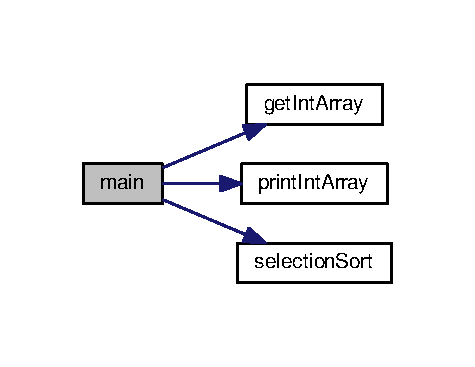
\includegraphics[width=228pt]{Selection_8c_a840291bc02cba5474a4cb46a9b9566fe_cgraph}
\end{center}
\end{figure}


\index{Selection.\+c@{Selection.\+c}!print\+Int\+Array@{print\+Int\+Array}}
\index{print\+Int\+Array@{print\+Int\+Array}!Selection.\+c@{Selection.\+c}}
\subsubsection[{\texorpdfstring{print\+Int\+Array(int n, int a[])}{printIntArray(int n, int a[])}}]{\setlength{\rightskip}{0pt plus 5cm}void print\+Int\+Array (
\begin{DoxyParamCaption}
\item[{int}]{n, }
\item[{int}]{a\mbox{[}$\,$\mbox{]}}
\end{DoxyParamCaption}
)}\hypertarget{Selection_8c_a8f37fcbee658573c44964f9271a48d5d}{}\label{Selection_8c_a8f37fcbee658573c44964f9271a48d5d}
\index{Selection.\+c@{Selection.\+c}!print\+Int\+Array@{print\+Int\+Array}}
\index{print\+Int\+Array@{print\+Int\+Array}!Selection.\+c@{Selection.\+c}}
\subsubsection[{\texorpdfstring{print\+Int\+Array(int n, int a[n])}{printIntArray(int n, int a[n])}}]{\setlength{\rightskip}{0pt plus 5cm}void print\+Int\+Array (
\begin{DoxyParamCaption}
\item[{int}]{n, }
\item[{int}]{a\mbox{[}n\mbox{]}}
\end{DoxyParamCaption}
)}\hypertarget{Selection_8c_a5ea4efa90d2fa03117a98b554d75be66}{}\label{Selection_8c_a5ea4efa90d2fa03117a98b554d75be66}

\begin{DoxyCode}
42 \{
43   \textcolor{keywordtype}{int} i;
44 
45   \textcolor{keywordflow}{for} (i=0; i<n; )\{
46     printf(\textcolor{stringliteral}{"\(\backslash\)t%d "}, a[i++]);
47     \textcolor{keywordflow}{if} (i%5==0)
48       printf(\textcolor{stringliteral}{"\(\backslash\)n"});
49   \}
50   printf(\textcolor{stringliteral}{"\(\backslash\)n"});
51 \}
\end{DoxyCode}
\index{Selection.\+c@{Selection.\+c}!selection\+Sort@{selection\+Sort}}
\index{selection\+Sort@{selection\+Sort}!Selection.\+c@{Selection.\+c}}
\subsubsection[{\texorpdfstring{selection\+Sort(int n, int a[])}{selectionSort(int n, int a[])}}]{\setlength{\rightskip}{0pt plus 5cm}void selection\+Sort (
\begin{DoxyParamCaption}
\item[{int}]{n, }
\item[{int}]{a\mbox{[}$\,$\mbox{]}}
\end{DoxyParamCaption}
)}\hypertarget{Selection_8c_acc86466d0607ef8c19c7d748904206e7}{}\label{Selection_8c_acc86466d0607ef8c19c7d748904206e7}

\begin{DoxyCode}
77 \{
78   \textcolor{keywordtype}{int} lcv;
79   \textcolor{keywordtype}{int} rh;      \textcolor{comment}{/*Elements in interval rh..n-1 are in their final position*/}
80   \textcolor{keywordtype}{int} where;   \textcolor{comment}{/*Position where we have current maximum*/}
81   \textcolor{keywordtype}{int} temp;    \textcolor{comment}{/*Used for swapping*/}
82   
83   \textcolor{keywordflow}{for}(rh=n-1;rh>0;rh--)\{
84     \textcolor{comment}{/*Find position of largest element in range 0..rh*/}
85     where = 0;
86     \textcolor{keywordflow}{for} (lcv=1;lcv<=rh;lcv++)
87       \textcolor{keywordflow}{if} (a[lcv]>a[where])
88     where = lcv;
89     temp = a[where];
90     a[where] = a[rh];
91     a[rh] = temp;
92   \}
93 \}\end{DoxyCode}

%--- End generated contents ---

% Index
\backmatter
\newpage
\phantomsection
\clearemptydoublepage
\addcontentsline{toc}{chapter}{Index}
\printindex

\end{document}
